\chapter{Stochastic Differential Equations}
\label{ch:SDE}
In this chapter we will define what we mean when we say that \(X_t\) is a \emph{solution} (or \emph{solution process}) of a stochastic differential equation and we will discuss the conditions under which the solution exists and its uniqueness. Furthermore we will give some examples of stochastic differential equations which can be solved analytically.
\section{Existence and uniqueness of solutions}
\begin{definition}[Stochastic differential equation]
Let a:\(\mathbb{R}\times[0,T]\to\mathbb{R}\) and b:\(\mathbb{R}\times[0,T]\to\mathbb{R}\) be measurable functions.
A stochastic differential equation (SDE) has the following form:
\begin{flalign*}
\text{SDE}\quad\begin{cases} \mathrm{d}X_t = a(X_t,t)\mathrm{d}t + b(X_t,t)\mathrm{d}W_t \\ 
X_0 = x_0\:\:\text{(initial value)}  \\
\end{cases}
\end{flalign*} 
for \(t\in[0,T]\). We will give it the following (It\^o-)representation:
\[X_t = x_0 + \int_0^t \!a(X_s,s)\,\mathrm{d}s + \int_0^t \!b(X_s,s)\,\mathrm{d}W_{s} \quad\text{P-a.s.}\]
and the following has to hold:
\begin{enumerate}[noitemsep,topsep=0mm,labelindent=6mm,leftmargin=*,widest=3.,align=right]
\item \(x_0\) is \(\mathcal{F}_0\)-measurable and \(\mathbb{E}[|x_0|^2]<\infty\:\:\)(can be constant). 
\item \(a(X_t,t)\) and \(b(X_t,t)\) as in definition \ref{Itoprocess}.
\end{enumerate}
\end{definition}
\begin{lemma}[Existence and Uniqueness]
\label{lemma:ExUn}
Given a stochastic differential equation as before. The solution \(X_t\) exists and is unique (P-a.s) if there are constants C, L \(\in\mathbb{R}\) s.t:
\begin{enumerate}[noitemsep,topsep=0mm,labelindent=6mm,leftmargin=*,widest=3.,align=right]
\item \(|a(x,t) - a(y,t)| \leq L|x-y| \\
	    |b(x,t) - b(y,t)| \leq L|x-y|\:\: \forall x,y\in\mathbb{R}, t\in[0,T] \:\:\text{(globally Lipschitz)} \) 	
\item \(|a(x,t)| \leq C(1+|x|) \\
	    |b(x,t)| \leq C(1+|x|)\:\:  \forall x\in\mathbb{R}, t\in[0,T] \:\:\text{(linear growth-bound)}\)
\end{enumerate}
In the autonomous case, where \(a(x,t) = a(x)\) and \(b(x,t) = b(x)\), the Lipschitz-condition implies the second condition.
\end{lemma}
\begin{proof}
See \cite{Oksendal}.
\end{proof}
\section{Analytically solvable equations}
There are not many stochastic differential equations which have an analytical (closed-form) solution. We will present the \emph{geometric Brownian motion} and the \emph{Ornstein-Uhlenbeck process} which have applications in physics and mathematical finance. Both are solutions of stochastic differential equations.
Knowing the exact solution allows us to test how good our approximation schemes are using simulation. This will be the subject of chapter \ref{ch:Num}.
\label{sec:}
\subsection{Geometric Brownian motion}
\begin{proposition}[Geometric Brownian motion]
The stochastic differential equation is given by:
\begin{flalign*}
& \mathrm{d}X_t = \mu X_t\mathrm{d}t + \sigma X_t\mathrm{d}W_t,\quad t\in[0,T],\quad X_0 = x_0\\
& X_t = x_0 + \int_0^t \!\mu X_s\,\mathrm{d}s + \int_0^t \!\sigma X_s\,\mathrm{d}W_{s} \quad\text{P-a.s.}
\end{flalign*}
where \(x_0\), \(\mu\), \(\sigma\:\in\mathbb{R}\) constant and \(\sigma>0\).
Its solution is:
\[X_t = x_0\exp({(\mu-\frac{\sigma^2}{2})t + \sigma W_t}).\]
\end{proposition}
If we set \(x_0=1\), then \(X_t\sim\exp (Z_t)\) where \(Z_t\sim\mathcal{N}((\mu - \frac{1}{2}\sigma^2)t, \sigma t)\). This means that \(X_t\) is lognormally distributed \(\forall\; t\in[0,T]\).
\begin{proof}
See example \ref{ex:gbm} and take the exponent. 
\end{proof}
\begin{figure}[!htbp]
\centering
  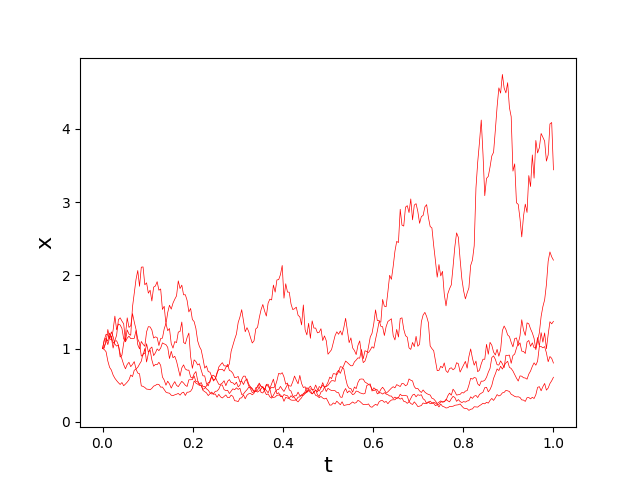
\includegraphics[scale=0.4]{content/Graphics/Figure_SamplingGBM.png}
  \caption{5 samples of the geometric Brownian motion with \(x_0 = 1, \mu = 1, \sigma = 1.5\).}
  \label{fig:}
\end{figure}

\subsection{Ornstein-Uhlenbeck process}
\begin{proposition}[Ornstein-Uhlenbeck process]
The stochastic differential equation is given by:
\begin{flalign*}
& \mathrm{d}X_t = -\beta X_t\mathrm{d}t + \sigma\mathrm{d}W_t,\quad t\in[0,T],\quad X_0 = x_0\\
& X_t = x_0 + \int_0^t \!-\beta X_s\,\mathrm{d}s + \int_0^t \!\sigma\,\mathrm{d}W_{s} \quad\text{P-a.s.}
\end{flalign*} 
where \(\beta\), \(\sigma\in\mathbb{R}\) constant and \(\beta\), \(\sigma>0\). We will choose \(x_0\) either to be constant or a normal-distributed random variable.
Its solution is:
\[X_t = x_0\exp({-\beta t}) + \sigma\int_0^t \!\exp({-\beta(t-s)})\,\mathrm{d}W_{s}.\]
\end{proposition} 
However we are not able to simulate the stochastic integral \(\int_0^{t_n} \!\,\exp({-\beta(t_n-s)})\,\mathrm{d}W_{s}\) exactly given the time step \(t_n\).
We will use the following approximation and consider it as the exact solution, given a partition \(P_n\) and a discretized Wiener process: 
\(\sum^{n-1}_{k=0}\exp({-\beta(t_n-t_k)})(W_{t_{k+1}}-W_{t_k})\).
\begin{proof}
Again we will use It\^o's lemma: Let u: \((x,t)\mapsto\ x\exp({\beta t})\). Then
\begin{flalign*}
& u_x(x,t) = \exp({\beta t}),      \:\:u_{xx}(x,t) = 0, \:\:u_{t}(x,t) =  x\beta\exp({\beta t})\\
& u(X_t,t)-u(X_0,0) = \int_0^t \!u_t(X_s,s) - \beta X_s\cdot u_x(X_s,s)  + \frac{1}{2}u_{xx}(X_s,s)\sigma^2\,\mathrm{d}s + \int_0^t \!\sigma u_x(X_s,s)\,\mathrm{d}W_{s} \\
& X_t\exp({\beta t}) - X_0\exp({\beta 0}) = \int_0^t \!\beta X_s\exp({\beta s}) - \beta X_s\exp({\beta s}) + 0 \,\mathrm{d}s + \int_0^t \!\sigma\exp({\beta s})\,\mathrm{d}W_{s} \\
%& X_t\exp({\beta t}) = x_0 + \int_0^t \!\sigma\exp({\beta s})\,\mathrm{d}W_{s} \\
& X_t =  x_0\exp({-\beta t}) + \sigma\int_0^t \!\exp({-\beta(t-s)})\,\mathrm{d}W_{s}.
\end{flalign*}
\end{proof}
\begin{figure}[H]
\centering
  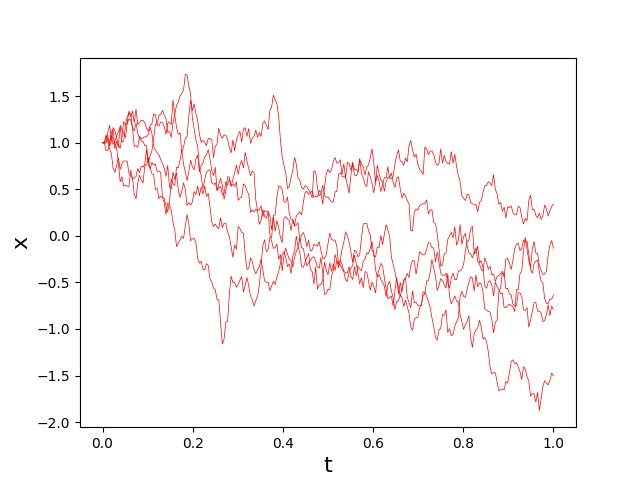
\includegraphics[scale=0.4]{content/Graphics/Figure_SamplingOU.png}
  \caption{5 samples of the Ornstein-Uhlenbeck process with \(x_0 = 1 , \beta = 1, \sigma = 1.5\).}
  \label{fig:}
\end{figure}


























